\documentclass{article}

\usepackage{enumitem}
\usepackage{amsmath}
\usepackage{amsfonts}
\usepackage{amssymb}
\usepackage{textcomp}
\usepackage{gensymb}
\usepackage[margin=0.5in]{geometry}
\usepackage[hidelinks]{hyperref}

\usepackage{tkz-berge}

\let\oldemptyset\emptyset
\let\emptyset\varnothing

\usepackage{environ}
\NewEnviron{centerframebox}{\begin{center}\fbox{\parbox{0.92\textwidth}{\BODY}}\end{center}}

\usepackage[many]{tcolorbox}
\newtcolorbox{cross}{blank,breakable,parbox=false,
  overlay={\draw[red,line width=5pt] (interior.south west)--(interior.north east);
    \draw[red,line width=5pt] (interior.north west)--(interior.south east);}}

\newcommand{\N}{\mathbb{N}}

\title{Combinatorial Optimization \\ Exercise Set 1}
\author{
  AAAAAAAAAA AAAAAAA \\
  \href{mailto:AAAAAAAAAAAAAAAAAAAA}{AAAAAAAAAAAAAAAAAAAA}
  \and
  Carola Ley \\
  \href{mailto:s6caleyy@uni-bonn.de}{s6caleyy@uni-bonn.de}
  \and
  Bailee Zacovic \\
  \href{mailto:s38bzaco@uni-bonn.de}{s38bzaco@uni-bonn.de}
}

\begin{document}
  \maketitle

  \setcounter{section}{1}
  \subsection{Infinite counterexample to Hall's Theorem}
  \begin{centerframebox}
    Find an infinite counterexample to Hall's Theorem. More precisely:
    Find a bipartite graph $G = (A \dot\cup B,\, E)$ with $A \cong \N$, $B \cong \N$, and $|N(S)| \geq |S|$ for
    every $S \subseteq A$ and every $S \subseteq B$ such that $G$ does not contain a perfect matching.
  \end{centerframebox}

  For our graph to be a counterexample to Hall's Theorem it has to violate one of the two conditions,
  but in a sneaky infinite way, so that ``on paper'' it isn't violated, but in reality no perfect matching exists because of it.
  We can't do much with the first condition, about the size of each part of the graph being equal,
  because they are already fixed to have cardinality $\aleph_0$.
  So we have to look at the second condition, $|N(S)| \geq |S|$,
  and here we can abuse the fact that ``$\geq$'' is not very good with infinite cardinalities.
  As long as $|N(S)| = \aleph_0$ the set $S$ could be any size we want, and the condition will still be satisfied.
  So, if we include a vertex with an infinite number of neighbors, any subset that includes it will automatically satisfy the condition.

  \begin{center}
    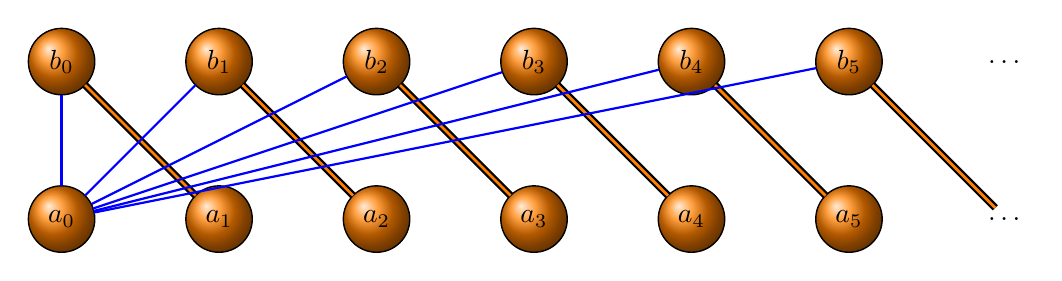
\begin{tikzpicture}
      \SetVertexMath
      \GraphInit[vstyle=Shade]

      \grEmptyPath[prefix=a,RA=2,RS=0]{6}
      \grEmptyPath[prefix=b,RA=2,RS=2]{6}

      \Edges(a1,b0)
      \Edges(a2,b1)
      \Edges(a3,b2)
      \Edges(a4,b3)
      \Edges(a5,b4)

      \node(a-dots) at (12,0) {$\dots$};
      \node(b-dots) at (12,2) {$\dots$};
      \Edges(b5,a-dots)

      \SetUpEdge[color=blue]
      \EdgeFromOneToAll{a}{b}{0}{6}
    \end{tikzpicture}
  \end{center}

  This graph is constructed as $V(G) = A \cup B$, where $A = \{a_i \mid i \in \N_0\}$ and $B = \{b_i \mid i \in \N_0\}$,
  as said in the formulation of the exercise.
  The edge set is also a combination of two parts: the edges leading to the $a_0$ node (here in blue),
  and the other edges connecting the two parts of the graph together.
  In set notation
  $E(G) = \{\{a_0,\, b_i\} \mid i \in \N_0 \} \cup \{\{a_{i+1},\, b_i\} \mid i \in \N_0 \}$.

  Now we have to check if it actually does satisfy the condition and that it doesn't have a perfect matching.
  If $S \subseteq B$ then $N(S) = \{a_0\} \cup \{a_{i+1} \mid b_i \in S\}$ and have cardinality
  $|N(S)| = |S|+1 \quad\to\quad |S|+1 \geq |S|$.
  If $S \subseteq A$ then we have to separately consider the cases of the special node $a_0$ being included or not.
  When it is included, the set of neighbors is just $B$ and has cardinality $\aleph_0$, so $\aleph_0 \geq |S|$ is always true.
  And when it is not included, the set of neighbors is $N(S) = \{b_{i-1} \mid a_i \in S\}$, where $i \geq 1$ by construction,
  and the cardinality of this set is $|N(S)| = |S|$.
  And that's all the cases.

  We also have to prove no perfect matching can exist in $G$.
  Assume there exists a perfect matching $M$.
  Then it has to contain an edge with the $a_0$ node: $\exists j : \{a_0, b_j\} \in M$.
  This means that $b_j$ cannot have any other edges in the matching and $\{b_j, a_{j+1}\} \notin M$.
  But this was the only edge linking $a_{j+1}$ to any other node, so it cannot be covered by the matching.
  And the matching isn't perfect!
  $\blacksquare$

  Note: $\N_0$ is the set of all natural numbers, including zero. $\aleph_0$ is the cardinality of this set.
  The words ``Node'' and ``Vertex'' are used interchangeably.

  \subsection{Bipartite graph}
  \begin{centerframebox}
    Let $G$ be a bipartite graph.

    \begin{enumerate}[label=(\alph*)]
      \item
      Let $V(G) = A \dot\cup B$ be a bipartition of $G$.
      If $A' \subseteq A$ and $B' \subseteq B$, and there are a matching $M_{A'}$ covering $A'$ and a
      matching $M_{B'}$ covering $B'$, show that there must be a matching that covers $A' \cup B'$.

      \item
      Suppose that for every non-empty $E' \subseteq E(G)$ we have $\tau(G - E') < \tau(G)$.
      Show that $E(G)$ is a matching in $G$.
    \end{enumerate}

    By $\tau(G)$ we denote the minimum cardinality of a vertex cover of $G$.
  \end{centerframebox}

  \subsubsection*{(a) Matchings}
  % \begin{cross}
  %   For matching $M_{A'}$ we create a subgraph $G_{A'} \subseteq G$ which excludes all vertices not covered by $M_{A'}$.
  %   $M_{A'}$ becomes a perfect matching in $G_{A'}$, and by Hall's Theorem we know that $|A'| = |V(G_{A'}) - A'| = |B''|$ (let $B'' = V(G_{A'}) - A'$)
  %   and $\forall S \subseteq V(G_{A'}) : |N_{A'}(S)| \geq |S|$.
  %   Note that the neighbor counting function $N_{A'}$ is different here, it only counts the neighbors in the $G_{A'}$ subgraph,
  %   but it will always be at least the amount of neighbors in the full graph $G$,
  %   so we can extend the inequality $|N(S)| \geq |N_{A'}(S)| \geq |S|$.
  %   And we can say $\forall S \subseteq A' : |N(S)| \geq |S|$, and, by analogy, the same for $B'$ (and $A''$ and $B''$).

  %   Without loss of generality, we can assume $A = A' \cup A''$ and $B = B' \cup B''$ so our graph doesn't contain any unused vertices.
  %   And also $E = M_{A'} \cup M_{B'}$, because no other edges are guaranteed to exist.
  % \end{cross}

  Let's construct a subgraph $G' \subseteq G$, such that it only contains the nodes and edges we care about,
  i.e. the ones that are involved with the two matchings we were given.
  So the edges $E(G') = M_{A'} \cup M_{B'}$ are just the union of our two matchings,
  and the vertices $V(G') = \{v \mid \exists e \in E(G') : v \in e \} $ are just the ones involved in the edges.
  The vertex set will also contain the $A'$ and $B'$ subsets, as well as their union $A' \cup B'$,
  because they are fully covered by $M_{A'}$ and $M_{B'}$ respectively.
  This graph will also remain bipartite.

  Every vertex in the reduced graph $G'$ will have degree 1 or 2, because each edge has to come form either $M_{A'}$ or $M_{B'}$,
  and matchings cannot have a vertex appear more than once.
  This graph becomes a disjoint union of paths and even length cycles (odd length cycles are not allowed on bipartite graphs),
  because any more complex structure will require a degree 3 or above vertex.

  Even cycles and even paths can both be easily covered by a perfect matching just by selecting every second edge.
  \begin{center}
    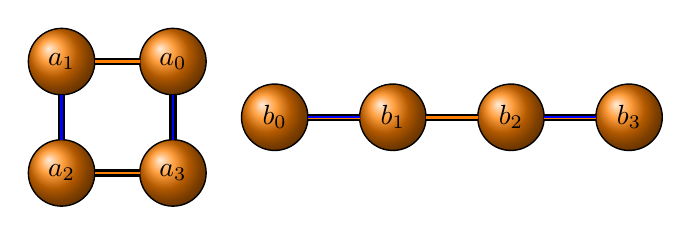
\begin{tikzpicture}
      \SetVertexMath
      \GraphInit[vstyle=Shade]
      \grCycle[prefix=a,rotation=45,RA=1]{4}
      \begin{scope}[xshift=2cm]
        \grPath[prefix=b,RA=1.5]{4}
        \SetUpEdge[color=blue]
        \Edges(b0,b1)
        \Edges(b2,b3)
      \end{scope}

      \SetUpEdge[color=blue]
      \Edges(a1,a2)
      \Edges(a3,a0)
      % \EdgeFromOneToAll{a}{b}{0}{6}
    \end{tikzpicture}
  \end{center}
  But for odd length paths we have to consider which vertices lie inside $A' \cup B'$,
  and make a matching that excludes a vertex that we don't need.
  Note that every vertex with degree 2 must be in either $A'$ or $B'$, because it is included in both matchings,
  and this path alternates edges from $M_{A'}$ and from $M_{B'}$.
  Thus we have to exclude one of the ends, and the path contains the same amount of edges from both matchings.
  % And if it starts with an edge form $M_{A'}$, it will end with an edge from $M_{B'}$ (and vice versa, for $A$ and $B$ being swapped).
  % if the path starts it $A$, it will also have to end in $A$ (and vice versa for $B$).

  Let's draw this path as a directed graph.
  Edges from $M_{A'}$ will be pointed towards $B$, and edges from $M_{B'}$ will be pointed towards $A$.
  \begin{center}
    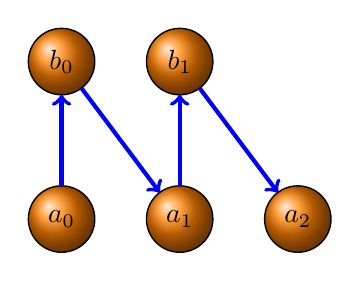
\begin{tikzpicture}
      \SetVertexMath
      \GraphInit[vstyle=Shade]
      \grEmptyPath[prefix=a,RA=1.5]{3}
      \grEmptyPath[prefix=b,RA=1.5,RS=2]{2}
      \SetUpEdge[lw = 1.5pt, color = blue]
      \tikzset{EdgeStyle/.style={->}}
      \Edges(a0,b0,a1,b1,a2)
    \end{tikzpicture}
  \end{center}
  This process will always produce a ``correct'' directed path, and vertices will be in $A' \cup B'$ iff they have an outgoing edge.
  So we can safely exclude the endpoint of this path, as it doesn't have an outgoing edge.

  So we have covered all the cases, and can now unify all of our small subgraph matchings,
  and the combination of them will always cover $A' \cup B'$.
  $\blacksquare$
  % cases: \\
  % 1) $A'' \cap A' = \emptyset$ and $B'' \cap B' = \emptyset$ -- easy \\
  % 2) $A'' = A'$ and $B'' = B'$ -- easy \\
  % 3)

  % bla bla bla \\
  % if we have $\forall S \subseteq C : |N(S)| \geq |S|$ and $\forall S \subseteq D : |N(S)| \geq |S|$
  % then what can we say about  $\forall S \subseteq C \cup D : |N(S)| \geq |S|$?
  % nothin???

  % counterexample:
  % A = {a_0, a_1}
  % B = {b_0, b_1}
  % A' = {a_0}
  % B' = {b_0}
  % E = {{a_0, b_1}, {a_1, b_0}}
  % M_{A'} = {{a_0, b_1}}
  % M_{B'} = {{a_1, b_0}}
  % A' \cup B' = {a_0, b_0}
  % did not work
  % TODO

  \subsubsection*{(b) Vertex covers}
  Let's define a notion of a vertex in a vertex cover \textit{covering} an amount of edges.
  In a vertex cover $C$ on graph $G$ a vertex $v \in C$ covers an edge $e \in E(G)$
  if this edge is no longer covered by $C \setminus \{v\}$.
  We can also sea, that if a vertex cover is minimal, then every vertex in it must cover at least one edge.
  And every edge must be covered by at least one vertex.

  If for every non-empty $E' \subseteq E(G)$ we have $\tau(G - E') < \tau(G)$,
  then removing any edge in the graph will make the minimal vertex cover have at least one less vertex.
  This means that the node that was covering that edge can be safely removed,
  i.e. it wasn't covering any other edges, because those still need to be covered.
  Also because the graph is bipartite and there are no odd length cycles, every edge can be covered by only one vertex.
  Applying it to the whole graph, we get that every node in that minimal vertex cover covers exactly one edge,
  and the size of the vertex cover will be the same as the number of edges $|C| = \tau(G) = |E(G)|$.
  % TODO: there's an error here. this doesn't hold in general for non bipartite graphs (addressed??)

  Using König's Theorem, on any bipartite graph the maximum matching size $\nu(G)$ is the same as minimum vertex cover size $\tau(G)$.
  So $|C| = \tau(G) = |E(G)| = \nu(G)$, and the maximum matching contains all the edges.
  Thus the set of all edges becomes a (perfect) matching.
  $\blacksquare$

  % unfinished note:
  % also if it contains a perfect matching, removing an edge outside of it will not reduce the vertex cover,
  % so the perfect matching (if it exists) must contain all the edges

  \subsection{Regular bipartite graph}
  \begin{centerframebox}
    Let $G$ be a $k$-regular bipartite graph.

    \begin{enumerate}[label=(\alph*)]
      \item
      Prove that $G$ contains $k$ disjoint perfect matchings. \\
      Hint: Use König's Theorem.

      \item
      Deduce from (a) that the edge set of any bipartite graph of maximum degree
      $k$ can be partitioned into $k$ matchings.
    \end{enumerate}

    A regular graph with vertices of degree $k$ is called a $k$‑regular graph.
  \end{centerframebox}

  % Kotya's version:
  % First we can use Hall's Theorem again to prove that this graph has a perfect matching.
  % Consider the subset $S$ (of only one of the parts of the bipartite graph) and its neighborhood $N(S)$.
  % Then the ``outgoing degree''
  % (to make explaining this easier, we pretend that this graph $G = (A \dot\cup B,\, E)$
  % is directed and all the edges point from $A$ to $B$, and $S \subseteq A$)
  % of $S$ is just the number of vertices in $S$ times $k$, i.e. $|S| \cdot k$.
  % Some of those edges may go to the same vertex,
  % but since all of our vertices have degree $k$ only at most $k$ of those ``outgoing'' edges can be directed at one vertex.
  % If we assume $|N(S)| < |S|$, then the nodes in $N(S)$ must handle all the outgoing edges from $S$,
  % but they can all handle at most $k \cdot |N(S)|$ edges which is less than $k \cdot |S|$,
  % so we get a contradiction and Hall's condition must be true for all subsets of $A$ and $B$.

Denote $G=(A\dot\cup B, E)$. First, observe by $k$-regularity that the number of edges ``leaving'' $A$ is counted by $k|A|,$ while the number if edges ``entering'' $A$ is counted by $k|B|.$ These quantities must equal, hence it follows that $|A|=|B|.$ Secondly, we'd like to establish the Hall condition for $G$, so suppose, toward a contradiction, that for some $X\subseteq A,$ $|\Gamma(X)|> |X|.$ This can be restated as:

$$|\{\text{edges leaving }X\}|=k|X|>k|\Gamma(X)|=|\{\text{edges leaving }\Gamma(X)\}|\geq |\{\text{edges entering }X\}|,$$

which is a contradiction, hence $G$ has a perfect matching by Corollary 1.9\footnote{A bipartite graph $G = (A\dot\cup B,\, E)$
has a perfect matching if and only if $|A| = |B|$ and the Hall condition holds}. We now claim that $G$ contains $k$ disjoint perfect matchings, and we do so by induction on $k.$ When $k=1,$ $G$ has exactly one perfect matching, given by $E(G)$. Let $k>1,$ and let $M$ denote a perfect matching guaranteed by Corollary 1.9. Observe that $G'=(A\dot\cup B, E-M)$ is a $(k-1)$-regular bipartite graph, since exactly one edge in $M$ was incident to each $v\in A\dot\cup B.$ Then by our induction hypothesis, $G'$ contains $k-1$ disjoint perfect matchings, each disjoint from $M$ by construction. It follows that $G$ contains $(k-1)+1=k$ disjoint perfect matchings.

It remains to show that the edge set of any bipartite graph of max degree $k$ can be partitioned into $k$ matchings. To this end, fix $G=(A\dot\cup B,E)$ such a bipartite graph. We can obtain a $k$-regular bipartite graph $G'$ from G by adding additional edges and vertices. Without loss of generality, suppose $m:=|B|-|A|\geq 0$. Then let $V(G')=((A\cup \{a_1,\dots, a_m\})\dot\cup B)$. Next, for each $v\in B$ such that $d_v:=k-\text{deg}(v)>0,$ add edges $\{v,w_1\},\dots,\{v,w_{d_v}\}\notin E(G)$ for distinct $w_1,\dots,w_{d_v}\in A$ such that $\text{deg}(w_i)<k$ for all $1\leq i\leq d_v$. Such a collection of vertices necessarily exists in $A$ for each $v\in B$, otherwise we obtain

\begin{align*}|\{\text{edges entering }B\setminus\{v\}\}|&>k((|A|-d_v)(\text{deg}(v))+(k-1)(k-d_v)\\ &= k((|A|-d_v)(k-d_v))+(k-1)(k-d_v)\\&= k|A|+(\underbrace{kd_v}_{\geq k}-(\underbrace{k-d_v}_{< k})) \\&\geq  k|B|+1,\end{align*}which is a contradiction.

From this process, it is clear that the number of edges entering $A\cup \{a_1,\dots,a_m\}$ in $G'$ is exactly $k(|A|+m).$ Moreover, if some $w\in A\cup \{a_1,\dots,a_m\}$ were such that $\text{deg}(w)\neq k,$ then there would exist $w'\in A\cup \{a_1,\dots,a_m\}$ such that $\text{deg}(w')>k$. But this would mean either (1) $w'$ had degree larger than $k$ in $G$, or (2) at some point in the above process, a new edge was added between $w'$ and some $v\in B$ when $w'$ already had degree $k.$ Either case is a contradiction, hence the resulting bipartite graph $G'$ is $k$-regular.

Finally, it follows by the previous result that $G'$ admits $k$ disjoint perfect matchings, label them $M_1,\dots,M_k$, such that $E(G')=M_1\cup \dots \cup M_k.$ Then $M_1\cap E(G),\dots ,M_k\cap E(G)$ is a collection of $k$ disjoint matchings in $G.$ So the claim holds. $\blacksquare$

%else

%$$|\{\text{edges leaving }A\}|>k|A|-d_v=k|B|-d_v\geq |\{\text{edges leaving } B\}|=|\{\text{edges entering } A\}|,$$

%which is a contradiction.



  \subsection{Stable set and edge cover}
  \begin{centerframebox}
    Let $\alpha(G)$ denote the size of a maximum stable set in $G$, and $\zeta(G)$ the minimum cardinality of an edge cover.

    \begin{enumerate}[label=(\alph*)]
      \item $\alpha(G) + \tau(G) = |V(G)|$ for any graph $G$,
      \item $\nu(G) + \zeta(G) = |V(G)|$ for any graph $G$ with no isolated vertices,
      \item $\zeta(G) = \alpha(G)$ for any bipartite graph $G$ with no isolated vertices.
    \end{enumerate}

    By $\tau(G)$ we denote the minimum cardinality of a vertex cover of $G$.
    By $\nu(G)$ we denote the maximum cardinality of a matching of $G$.
    A stable set $S$ of a graph $G = (V,\, E)$ is a set of pairwise non-adjacent vertices,
    i.e. no edge connects vertices in $S$.
  \end{centerframebox}
  % point (a) is stated directly in https://en.wikipedia.org/wiki/Vertex_cover#Properties
  % these are the Gallai Theorems
  % https://core.ac.uk/download/pdf/82186318.pdf

\subsubsection*{(a) $\alpha(G) + \tau(G) = |V(G)|$ for any graph $G$}
Let $S\subseteq V(G)$ be a maximum stable set in $G$, so $|S|=\alpha(G)$. By the definition of a stable set every edge in $G$ has at most one vertex in $S$ and therefore at least one vertex in $V(G)\setminus S$, so $V(G)\setminus S$ is an vertex cover and we know $\alpha(G) + \tau(G)\leq |S|+ |V(G)\setminus S|= |V(G)|$.

Suppose there is an minimum vertex cover $T\subseteq V(G)$ with $|T|<|V(G)\setminus S|$, then as $T$ covers all edges, $V(G)\setminus T$ is a stable set with size $|V(G)\setminus T|>|S|$, which is a contradiction to $S$ being a maximum stable set. Thus $V(G)\setminus S$ is a minimum vertex cover with size $|V(G)\setminus S|=\tau(G)$ and therefore $\alpha(G) + \tau(G)= |S|+ |V(G)\setminus S| = |V(G)|$. $\blacksquare$

\subsubsection*{(b) $\nu(G) + \zeta(G) = |V(G)|$ for any graph $G$ with no isolated vertices}
Let $G$ be a graph with no isolated vertices.

If $G$ contains a perfect matching $M\subseteq E(G)$, then it is also a minimum edge cover and thus $\nu(G)=\zeta(G)=|M|=\frac{|V(G)|}{2} \Rightarrow \nu(G) + \zeta(G)= 2 \frac{|V(G)|}{2} = |V(G)|$.

Otherwise $G$ has no perfect matching. Let $M$ be a maximum matching in $G$  with size $|M|=\nu(G)$. Let $M'$ be a copy of $M$. For every vertex $v\in V(G)$ that is not covered by $M$, add one incident edge $\{v,u\}\in E(G)$ to $M'$. Such an edge always exists as there are no isolated vertices and the other vertex $u$ of the edge is already covered by $M$, as otherwise there would be a larger matching than $M$. This new set $M'$ covers all vertices of $G$, thus $\zeta(G)\leq|M'|=|M|+(|V(G)|-2|M|)=|V(G)|-|M|$.

Suppose there is an minimum edge cover $C$ with $|C|<|M'|$. As it is minimum, there are only paths of length 1 or 2 in $(V(G), C)$. The total number of vertices covered by $M'$ and $C$ are the same, so $C$ has less paths of length 2 and more of length 1 than $C$. As one can construct a matching in $G$ by taking one edge of each path in $C$, there is a matching with more edges than $M$, which is a contradiction to $M$ being a maximum matching. Thus $\zeta(G)=|M'|=|V(G)|-|M|=|V(G)| -\nu(G) \Leftrightarrow \nu(G) + \zeta(G) = |V(G)|$. $\blacksquare$

\subsubsection*{(c) $\zeta(G) = \alpha(G)$ for any bipartite graph $G$ with no isolated vertices}
Let $G$ be an bipartite graph with no isolated vertices. As $G$ is bipartite König’s Theorem gives us $\nu (G)=\tau(G)$. As $G$ has no isolated vertices, from part (a) and (b) we know $\alpha(G) + \tau(G) = |V(G)|= \nu(G) + \zeta(G)$. Thus with König's Theorem $\alpha(G) + \tau(G) = \nu(G) + \zeta(G) \Rightarrow \alpha(G) = \zeta(G)$. $\blacksquare$


\end{document}
